\chapter{System Overview}
\label{chp:system-overview}

\section{Vector Graphics in Hardware}

This section gives an overview of how vector graphics is represented in the \vthreek architecture.
Later sections describe how the architecture processes and produces output based on this representation.

\subsection{Primitives}

The \vthreek architecture supports 3 basic primitives: lines, quadratic Bézier curves and cubic Bézier curves.
Lines are represented as linear Bézier curves.

\begin{figure}[h!]
    \centering
    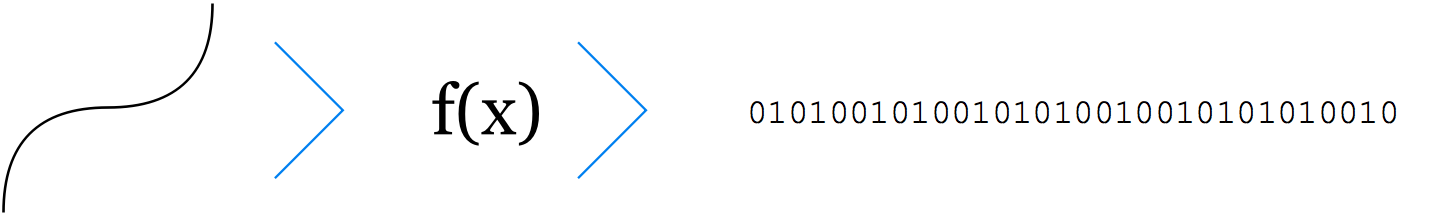
\includegraphics[width=0.85\linewidth]{images/primitive_encoding.png}
    \caption{Deciding upon an encoding scheme for vector primitives was one of the first decisions the group had to make.}
    \label{fig:primitive_encoding}
\end{figure}

Each primitives type is identified by the eight first bits.
To store a position on the screen, 32 bits is required: 16 bit for X and 16 bit for Y.
A line is represented by a start point and an end point.
To represent a quadratic Bézier curve a total of three points are needed, a start point, a control point and an end point.
The cubic Bézier curve includes one extra control point compared to the quadratic curve.
Table \ref{tbl:primitives} illustrates how each primitive is encoded as a binary string.

With the basic primitives linear, quadratic, and cubic Bézier curves, most other shapes can be constructed.
A square can be represented as four lines, a circle as multiple Bézier curves, and so on.

\begin{table}[h]
    \centering
    \begin{tabularx}{\linewidth}{|l|X|X|X|X|X|X|X|X|X|}
    \hline
    Primitive type (8) & x (16) & y (16) & x (16) & y (16) & x (16) & y (16) & x (16) & y (16) & Total bits \\ \hline
    Linear Bézier    & \(p_0^x \) & \(p_0^y \) & \(p_1^x \) & \(p_1^y \) & ~   & ~   & ~   & ~   & 72    \\ \hline
    Quadratic Bézier & \(p_0^x \) & \(p_0^y \) & \(p_1^x \) & \(p_1^y \) & \(p_2^x \) & \(p_2^y \) & ~   & ~   & 104   \\ \hline
    Cubic Bézier     & \(p_0^x \) & \(p_0^y \) & \(p_1^x \) & \(p_1^y \) & \(p_2^x \) & \(p_2^y \) & \(p_3^x \) & \(p_3^y \) & 136   \\ \hline
  \end{tabularx}
    \caption{Binary encoding of primitives. Bit size in parenthesis.}
	\label{tbl:primitives}
\end{table}

\subsection{Vector Images}

A vector image, or a scene, is a 2D canvas of fixed width and height on which primitives are placed.
The \vthreek architecture represents a scene conceptually as a collection of primitives.
Since primitives are represented with 16-bit integer coordinate-components, scene dimension is $65535 * 65535$.
This conceptual representation maps to a 1024 word deep, 136 bit wide, dual port scene memory module implemented using block RAM \cite{xilinx-block-ram} on the FPGA.
Since the size of the scene memory is static, the architecture maintains a primitive counter, indicating how many primitives are actually in the scene at any given time.


\section{Architectural structure}

\begin{figure}[H]
    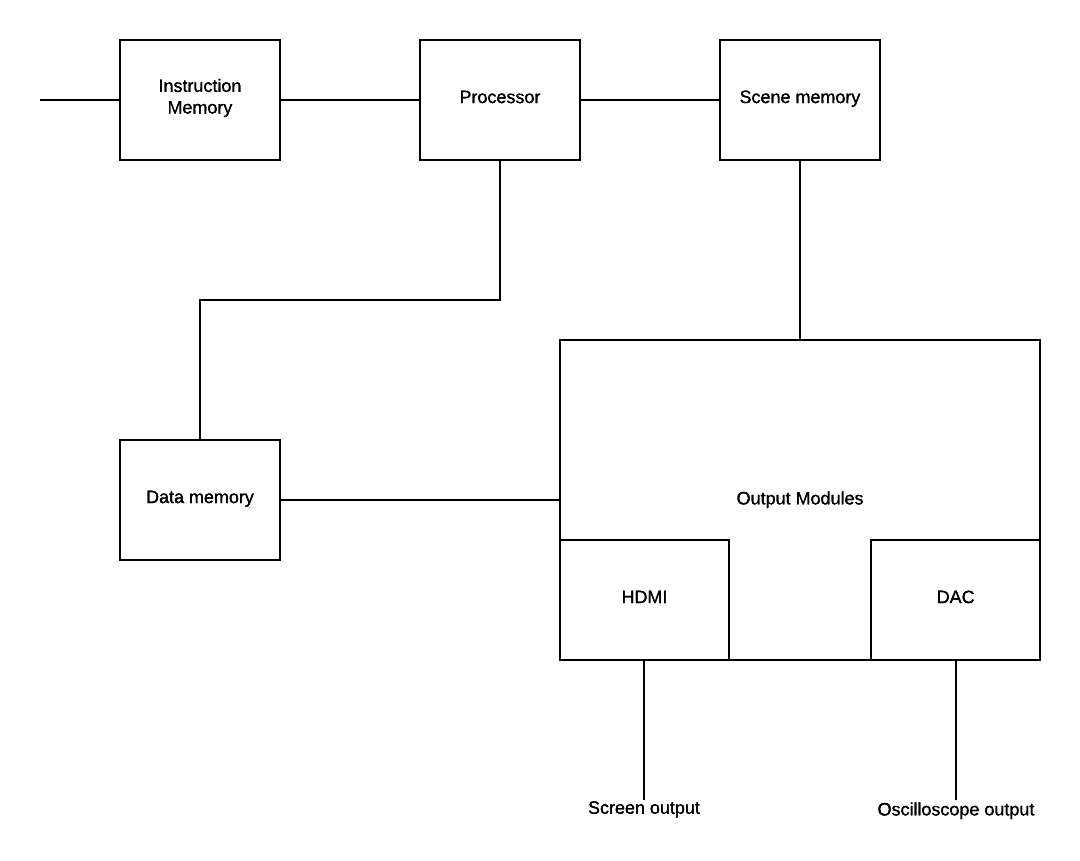
\includegraphics[width=\linewidth]{images/system-overview.png}
    \caption{A logical overview of the \vthreek architecture}
    \label{fig:system-overview}
\end{figure}

Figure \ref{fig:system-overview} shows how the major building blocks of the \vthreek architecture come together on a conceptual level.
Separation of instruction and data memory makes it a Harvard-like architecture \cite{structured-computer-organization}.
The processor reads from instruction memory, executes instructions and adds/updates vector primitives in the scene memory.
Preprocessing these primitives for output is done by the output modules.

\section{Programming Model}
\label{sec:programming-model}

While the primary goal of the \vthreek architecture is to provide efficient means of working with vector graphics, it is also designed with approachability in mind.
The parts of the programming model that are not directly related to vector operations, should be familiar to any developer used to other modern \gls{risc}-like architectures.

From the programmers point of view, there are two separate memories available; the general data memory and the scene memory.
The processor provides 32 general purpose 32-bit registers.
A special purpose 136-bit primitive register is provided as the main interface through which primitives are created and modified.

\subsection{Available Instructions}

The \vthreek \gls{isa}, described in appendix \ref{app:isa}, defines instructions both for general computation and special purpose instructions for working with primitives and the scene.
General purpose instructions are outlined briefly here, while vector instructions are elaborated on in greater detail.

\subsubsection{General}

As per the requirements \ref{sec:requirements}, the \vthreek processor is designed to be general.
In other words, it supports integer arithmetic, reading from and writing to data memory and conditional branching.

Working with the data memory is supported through the \texttt{ldr} and \texttt{str} instructions.
They share the same syntax, namely \texttt{<op> <register> \#<address>}.
For \texttt{ldr}, the register is the register in which the data at the address should be stored.
Similarily, for \texttt{str}, the data in the register is stored at the address.

Moving data into registers can also be done using the \texttt{mov}, \texttt{movl} and \texttt{movu} instructions.
Since both registers and instructions are 32 bits, all values that are possible to store in registers can't be encoded into an instructions.
Move instructions share the same syntax, \texttt{<op> <register> \#<16-bit immediate>}.
\texttt{mov} sets the upper 16 bits of the specified register to zero and the lower 16 bits to the immediate value.
\texttt{movl} sets the lower 16 bits of the register to the specified value, leaving the upper 16 bits unchanged, and \texttt{movu} vice versa.

Branching is done conditionally with the \texttt{beq} instruction and unconditionally with \texttt{jmp}.
\texttt{beq} compares the contents of two registers and jumps to an offset (specified in the instruction) from the current program counter value if the contents are equal.
\texttt{jmp} jumps unconditionally to an address specified in the instruction.

The processor implements two arithmetic instructions, \texttt{add} and \texttt{lsl}.
In the context of arithmetic, operands are treated as signed values, so subtraction is also possible.
\texttt{add}, with syntax \texttt{add Rd, Rs, Rt}, adds the contents of registers \texttt{Rs} and \texttt{Rt} and stores the result in register \texttt{Rd}.
Logical shift left, with syntax \texttt{lsl Rd, Rs, <immediate>} shifts the contents of register \texttt{Rs} by a number of bits specified using a logical left shift.

\subsubsection{Vector Instructions}

Several instructions for working with primitives and the scene are available.
A new primitive is created by issuing a \texttt{line}, \texttt{bezquad} or \texttt{bezcube} instruction.
Linear, quadratic and cubic Bézier curves are defined by, respectively, two, three and four control points.
Each control point fits into a 32-bit register, with 16 bits per coordinate component.
Primitive coordinates are initialized into the special purpose primitive register using the following syntax:

\begin{lstlisting}[label=lst:primitive-initialization]
line Rs, Rt
bezquad Rs, Rt, Ru
bezcube Rs, Rt, Ru, Rv
\end{lstlisting}

Figure \ref{fig:primitive-data-mapping} shows how coordinate components are aligned in general purpose registers, ready to be used as a control point for a primitive.

\begin{figure}[H]
    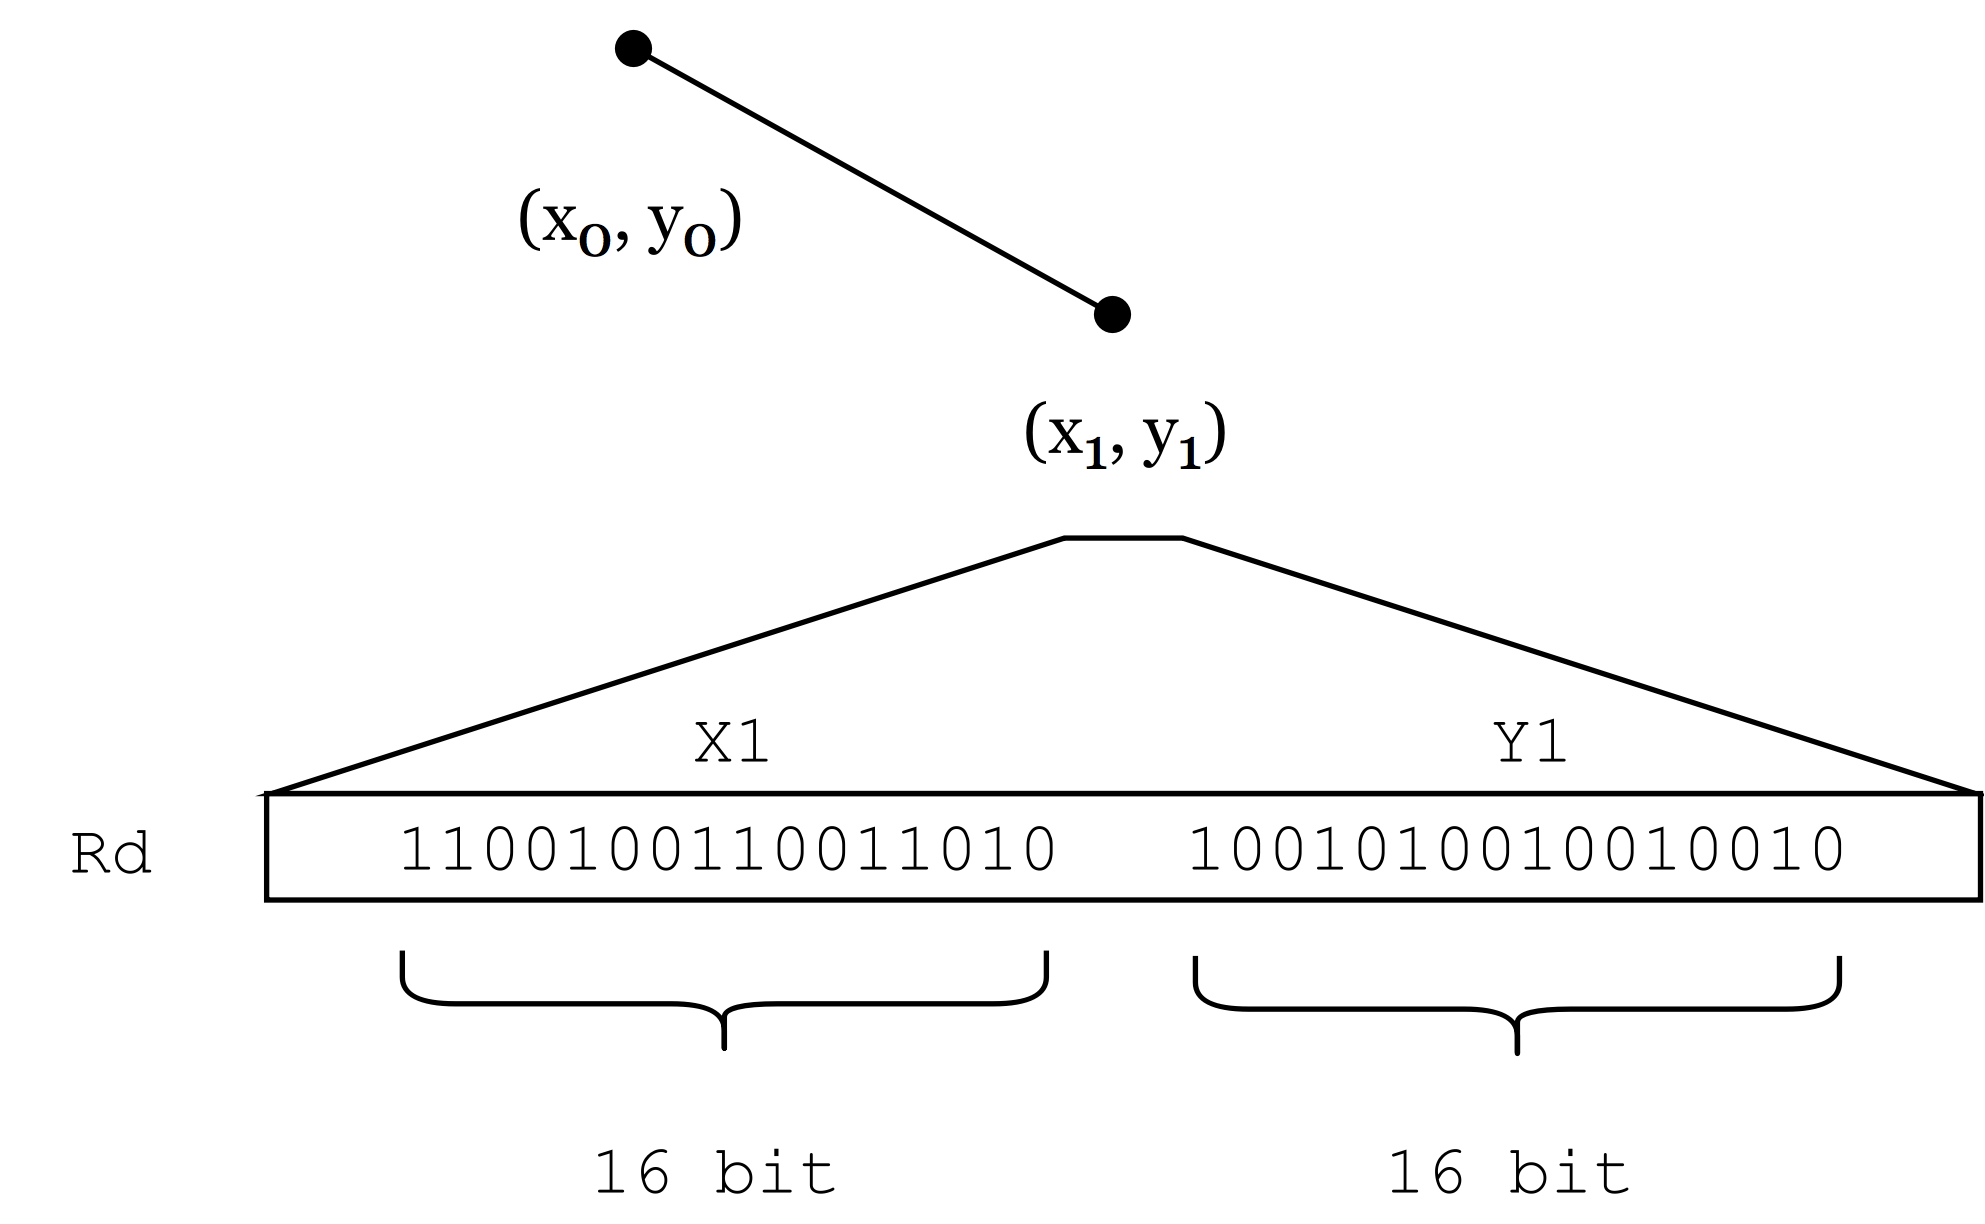
\includegraphics[width=\linewidth]{images/primitive-data-mapping.png}
    \caption{Mapping from x,y coordinates to 32-bit registers.}
    \label{fig:primitive-data-mapping}
\end{figure}

Once a primitive has been initialized it has to be written to the scene memory before it can be displayed.
This is done with the store primitive instruction, \texttt{strp}.
It takes a scene memory address as it's only argument.
\texttt{strp} also increments the primitive counter.

Once a primitive is in the scene memory, the output module will take care of producing display output.
A primitive can be read back into the processor core with the \texttt{ldrp} instruction, which similarily to \texttt{strp} takes an address as its only argument.
The instruction loads the primitive at the specified address in scene memory back into the primitive register in the processor core.

The primitive currently in the primitive register can be modified using getter and setter instructions.
\texttt{getpX Rd} copies the value of control point \texttt{X} into register \texttt{Rd}.
Inversely, \texttt{setpX Rs} sets the value of control point \texttt{X} in the primitive register to the value stored in register \texttt{Rs}.
When overwriting a primitive in scene memory, incrementing the primitive counter is often not desired.
Since \texttt{strp} does this implicitly, a separate instruction, \texttt{updp}, is provided.
It has the same syntax as \texttt{strp}, but does not increment the primitive counter.

\subsection{A Simple \vthreek Program}

\begin{lstlisting}[label=lst:simple-program]
mov r1, #0
movu r2, #-1
movl r2, #-1

line r1, r2
strp #0
\end{lstlisting}

Listing \ref{lst:simple-program} shows a very simple \vthreek program.
It simply draws a line across the scene, from bottom left corner to top right.

The first three lines store coordinates $0, 0$ and $65535, 65535$ in registers \texttt{r1} and \texttt{r2}.
Since values are treated as signed numbers in general purpose registers, but as unsigned in the context of vector primitives, $-1$ is used to indicate maximum value of a coordinate component.

A line with start-/endpoints as specified in \texttt{r1} and \texttt{r2}, is initialized into the primitive register on line four, and written to the scene memory on the next.

\subsection{More advanced programs}

A slightly more advanced program is listed in appendix \ref{app:tunnel}.
In addition to drawing static lines, it also showcases how animation can be performed using \texttt{beq} and \texttt{jmp}.


